\documentclass[11pt, ngerman, fleqn, DIV=15, headinclude, BCOR=2cm]{scrreprt}

\usepackage{../../header}

\usepackage{placeins}
%\usepackage[maxfloats=50]{morefloats}

\usepackage{csquotes}

\usepackage{tikz}
\usetikzlibrary{chains}
\usetikzlibrary{shapes.geometric}

\tikzset{device/.style={
                rectangle,
                minimum size=6mm,
                draw=black
            },
            monitor/.style={
                rectangle,
                rounded corners=2mm,
                minimum size=6mm,
                draw=black
            },
        }

\usepackage{pgfplots}
\pgfplotsset{
    compat=1.9,
    width=0.8\linewidth,
    xticklabel style={/pgf/number format/use comma},
    yticklabel style={/pgf/number format/use comma},
}
\usepgfplotslibrary{polar}

\usepgfplotslibrary{external}
\tikzexternalize[mode=list and make]
\tikzsetexternalprefix{Abbildung-}

\DeclareSIUnit{\skt}{SKT}

\usepackage{booktabs}

\hypersetup{
    pdftitle=
}

\newcommand{\plotwidth}{0.8\linewidth}

\subject{Praktikumsprotokoll}
\title{Compton-Effekt}
\subtitle{Versuch P526 -- Universität Bonn}
\author{
	Frederike Schrödel \\
	\small{\href{mailto:fschroedel@gmx.de}{fschroedel@gmx.de}}
	\and
	Simon Schlepphorst \\
	\small{\href{mailto:s2@uni-bonn.de}{s2@uni-bonn.de}}
}

\date{2015-11-10}

\publishers{Tutor: Peter Klassen
}

\begin{document}

\maketitle

\begin{abstract}
    In diesem Versuch beschäftigen wir uns mit der Wechselwirkung von
    $\gamma$-Strahlung in Materie, wobei wir uns besonders mit der
    Comptonstreuung beschäftigen.  Hierbei interessieren uns vor allem der
    totale Wirkungsquerschnitt und die Winkelabhängigkeit von Intensität und
    Energie der $\gamma$-Strahlung.
\end{abstract}

\tableofcontents

\chapter{Theorie}

%\section{Wechselwirkung von $\gamma$-Strahlung in Materie}
%Energiereiche Photonen, wie die zu betrachtenden $\gamma$-Teilchen können in
%Materie Wechselwirken. Hierbei hängt der dominierende Effekt von der
%Energie der Teilchen und der Ordnungszahl ab.
%TODO Skizze Wirkungsquerschnitt-energie 
%Im unteren Energiebereich, ab dem Punkt wo die Energie höher ist als die
%Bindungsernergie findet hauptsächlich der Photoeffekt statt. Im mittleren
%Bereich dominiert der Compten-Effekt und ab einer Energie von
%\SI{1022}{\kilo\electronvolt} kann auch vermehrt die Elektron-Positron-
%Paarbildung auf treten.
%%%%%%%%%%%%%%%%%%%%%%%%%%%%%%%%%%%%%%%%%%%%%%%%%%%%%%%%%%%%%%%%%%%%%%%%%%%%%%%%%

\section{Wechselwirkung von $\gamma$-Strahlung mit Materie}
\label{sec:WW-strahlung-Materie}

Die $\gamma$-Strahlung entsteht wenn nach einem vorhergegangen Zerfall der
Tochterkern nicht in seinen Grundzustand, sondern in einen angeregten Zustand
zerfällt.
Dieser angeregte Zustand zerfällt nach einiger Zeit durch Abstrahlung eines
$\gamma$-Quants in den Grundzustand. Diese Photonen sind sehr energiereich,
weshalb sie genug Energie haben, um auf verschiedene Weisen mit der Materie zu
wechselwirken. Hierbei hängt der dominierende Effekt von der
Energie der Teilchen und der Ordnungszahl des Wechselwirkungspartners ab.
%TODO Skizze Wirkungsquerschnitt-energie 
Im unteren Energiebereich, ab dem Punkt wo die Energie höher ist als die
Bindungsenergie, findet hauptsächlich der Photoeffekt statt. Im mittleren
Bereich dominiert der Compton-Effekt und ab einer Energie von
\SI{1022}{\kilo\electronvolt} kann auch vermehrt die
Elektron-Positron-Erzeugung auftreten.

Dabei darf aber nicht vergessen werden, dass es durchaus noch eine große
Wahrscheinlichkeit gibt, dass $\gamma$-Strahlung nicht wechselwirkt.


\subsection{Photoeffekt}
Der Photoeffekt beschreibt den Vorgang, bei welchem ein Photon ein Elektron aus
dem Atom auslöst.
Hierbei gibt das Photon seine komplette Energie ab.
Die kinetische Energie des ausgelösten Elektrons hängt nur über die
Bindungsenergie ($E_\text{Bind.}$) mit dem der Energie des Photons ($h\nu$),
also dessen Frequenz ($\nu$) zusammen.
Dieser Prozess kann nur in der Nähe eines Atomkerns stattfinden, weil dieser
den Rückstoß aufnimmt.
So bleibt bei diesen Vorgang Energie und Impuls erhalten. 
\[ 
    E = h\nu - E_\text{Bind.}
\]
Wenn man sich den Wirkungsquerschnitt $\sigma$ für diesen Prozess anschaut,
dann stellt man eine große Abhängigkeit von der Ordnungszahl $Z$ fest.
\[
    \sigma \propto Z^5 E_\gamma^{\frac 72}
\]
Deshalb tritt dieser Effekt besonders häufig bei Elementen mit hoher Ordnungszahl
auf.

 \subsection{Paarerzeugung}

Ein weiterer Effekt, der bei Energien $E_\gamma \ge 2m_\text ec^2$ auftreten
kann, ist die Elektron-Positron-Paarbildung.
Dieser Effekt ist allerdings erst ab weit oberhalb dieser Schwelle relevant.
Für den Wirkungsquerschnitt gilt $\sigma \propto Z^2$.


\subsection{Comptonstreuung}
Wenn Photonen an einem Elektron streuen, dann spricht man vom Comptoneffekt. 
Hierbei gibt das Photon einen Teil seiner Energie an das Elektron ab und ändert dabei
seine Frequenz.%TODO bild Comptonstreuung
Die abgegebene Energie hängt dabei vom Streuwinkel ab.
Für die Restenergie des Photons gilt:
\[
    E_\nu'(\phi) = \frac{E_\nu}{1+\frac{E_\nu}{m_\text ec^2}(1+\cos(\phi))}
\]
Die größte Energieänderung erhält man also bei einem Winkel von
$\phi=\SI{180}{\degree}$.
Diese Energieänderung berechnet sich durch:
\[
    \Delta\lambda = \frac{h}{m_\text ec}(1-\cos(\phi))
\]
Der Wirkungsquerschnitt entspricht $\sigma_\text C \propto \frac{Z}{E_\gamma}$.
%TODO nur für coptoneffekt
%TODO bild Spektrum im szintilator


\section{Wirkungsquerschnitte}
Hier muss zwischen dem differenziellen- und dem absoluten Wirkungsquerschnitt
unterschieden werden.
Die Herleitung für den Wirkungsquerschnitt des Comptoneffektes gelang unter
Nutzung der Dirac-Gleichung. Verantwortlich hierfür waren Nishina und
Klein, nach welchen auch die Darstellung, der Klein-Nishina-Plot, benannt ist.
\[
    \dod \sigma\Omega = \frac{r^2_\text{e}}{2}
    \frac{1}{(1+\gamma(1-\cos(\theta)))^2}\del{1+\cos(\theta)^2+\frac{\gamma^2(1-\cos(\theta)^2)}{1+\gamma(1-\cos(\theta))}}
\]
\label{eq:dif-querschnitt}
\ref{eq:dif-querschnitt} heißt Klein-Nishina Formel und beschreibt den
differenziellen Wirkungsquerschnitt mit dem Stoßwinkel $\theta$.
Um den totalen Wirkungsquerschnitt zu erhalten integriert man über den
Raumwinkel:
\[
    \sigma = 2\pi r^2_e
    \del{\frac{1+\gamma}{\gamma^2}\del{\frac{2(1+\gamma)}{1+2\gamma}-\frac
        1\gamma\ln(1+2\gamma)}+\frac
    1{2\gamma}\ln(1+2\gamma)-\frac{1+3\gamma}{(1+2\gamma)^2}}
\]
%Wenn man hieraus das Energiespektrum ermitteln möchte, so kann man in der
%Klein-Nishina-Formel 
%\[
%    \dod{\sigma}{T} = 
%    \frac{\pi r^2_\text e}{m_\text ec^2\gamma^2} \del{
%        2+\frac{s^2}{\gamma^2(1-s)^2}+\frac{s}{1-s}\del{s-\frac 2\gamma}}
%\]

Darstellen lässt sich die Winkelverteilung der Photonen durch den Wirkungsquerschnitt in einem
Klein-Nishina Plot. 

\begin{figure}
	\centering
	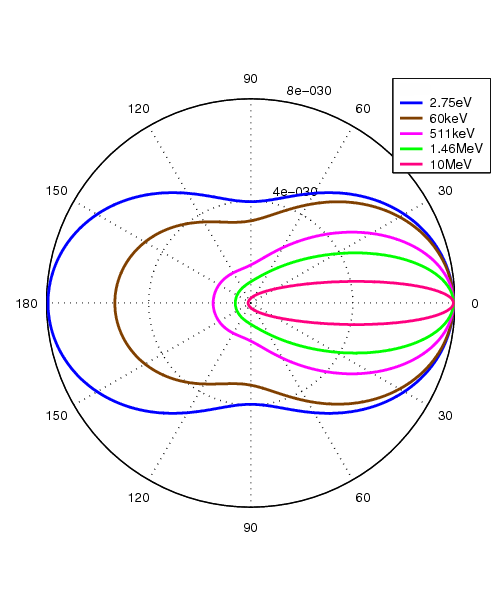
\includegraphics[width=0.65\textwidth]{../graphics/Klein-Nishina_distribution.png}
	\caption{%
		Klein-Nishina-Distribution aus \parencite{klein-nishina}
	}
\end{figure}

\section{Szintillationsdetektor}
Mit einem Szintillationsdetektor lassen sich Intensität und Energie von
ionisierender Strahlung messen.
Er besteht aus einem Szintillator und einem Photomultiplier.
Der Szintillator ist ein dotierter Einkristall, der von energiereicher
Strahlung zum Fluoreszieren angeregt werden kann und hinreichend
durchlässig für das von ihm emittierte Licht ist.

Innerhalb des vor äußerem Lichteinfall geschützten Szintillators entstehen durch
ionisierende Strahlung Lichtblitze. 
Diese entstehen dadurch, dass die Strahlung Atome durch die in Kapitel~\ref{sec:WW-strahlung-Materie}
beschriebenen Effekte anregt. Beim zurückfallen in den Grundzustand senden
diese dann wieder Photonen aus. Da die Anzahl der angeregten Atome von der
Energie der einfallenden Strahlung abhängt, ist die Intensität dieser Blitze
ebenfalls proportional zur Energie der einfallenden Strahlung.
%TODO nur für coptoneffekt? Bild Spektrum
%In dem entstehenden Spektrum, bei dem die Intensität gegen Energie
%aufgetragen. Man erhält ein Compton-Kontinuum, welches die Comptonstreuung bis
%zu einem Winkel von \SI{180}{\degree} enthält. Da bei diesem Wert der maximale
%Energieübertrag stattfindet, hat erhält man eine scharfe Kante, die Compton
%Kante. Wird nicht nur ein Teil der Energie abgegeben, wie es bei Photoeffekt
%der Fall ist, entsteht der energetisch höher gelegene Ausschlag. Man nennt
%ihn Photo-Peak.



\subsection{Photomultiplier}
Aufgrund des Photoeffektes, werden an der Photokathode des Photomultipliers
Elektronen ausgelöst.

Durch den Aufbau des Photomultipliers kommt es zu einem Lawineneffekt,
welcher die Elektronen vervielfacht und somit eine Detektion erleichtert.
Die Amplitude des so entstanden Strompulses ist somit auch proportional zu der
Energie der Eingangsstrahlung.
%TODO für Driftkammer
%Wenn man eine gute Energieauflösung möchte, sollte man allerdings eher einem
%Halbleiterdetektor nutzen.

\subsection{Energie und Zeitauflösung}
Um mit dieser Art Detektor möglichst gute Auflösungen zu erhalten, greift man
das Signal je nachdem ob man die Energie- oder die Zeitauflösung optimieren will
an eine Dynode beziehungsweise an der Anode des Photomultipliers ab.
Der Vorteil der Dynode für die Energieauflösung liegt da drin, dass noch keine
Sättigung herrscht. Hierdurch ist die Proportionalität zwischen Signalhöhe und
Energie nicht beeinträchtigt. Da das Signal allerdings nur sehr langsam
ansteigt, man spricht von den Slow-Signal, ist die Zeitauflösung beeinträchtigt.
Deswegen benutzt man dafür das sogenannte Fast-Signal. Es wird an der Anode
abgegriffen, da dort Sättigung vorliegt, wodurch das Signal schnell ansteigt.
Die Amplitude ist allerdings nicht mehr proportional zur Energie.
%Um die Zeitauflösung ermitteln zu können nutzt man eine
%Slow-Fast-Koinzidenzschaltung. Man misst bekannte Linien und bestimmt aus den
%angepassten Funktionen die Halbwertsbreite.
In diesem Versuch benutzen wie das Slow-Signal, da uns die Energie der
einfallenden Strahlung interessiert.

%TODO für Nukleare elektronik
%Für die Zeitkalibrirung nutzt man
%am besten ein Isotope, welches einen $\beta^+$-Zerfall besitzt. Dadurch kann
%man gewährleisten, dass gleichzeitig zwei Photonen mit bekannter Wellenlänge
%von \SI{511}{\ilko\electronenvot} durch die Rekombination von Elektron und
%Positron entstehen.

\subsection{Multi-Channel-Analyzer}
Um ein nach Amplituden sortiertes Spektrum zu erhalten, nutzen wir ein MCA.
Dies ist ein Bauteil, welches einkommende Signale nach Amplitude sortiert und
dann den Zähler im Kanal, welcher der Impulshöhe entspricht, hoch setzt. So erhalten wir ein
Histogramm.

%TODO Bild Spektrum
\begin{figure}
	\centering
	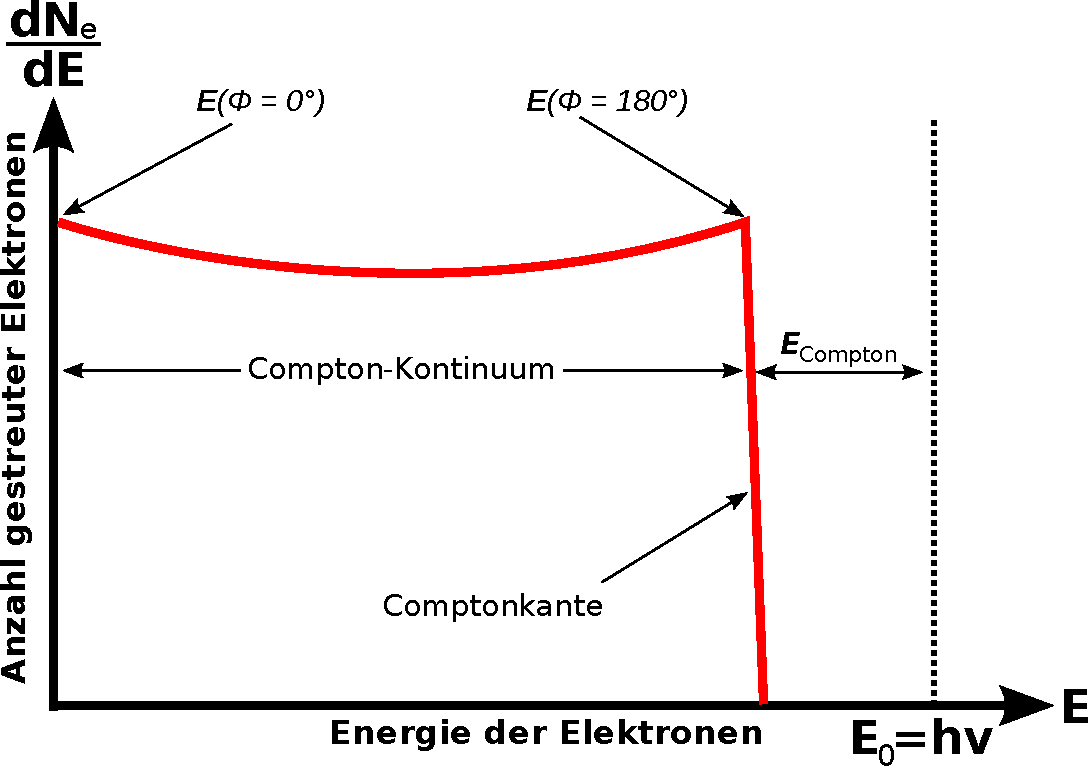
\includegraphics[width=0.6\linewidth]{../graphics/Compton-spektrum.pdf}
	\caption{%
		Spekrum mit dargestelltem Comptoneinfluss \parencite{comptoneffekt}
	}
	\ref{fig:compton-spektrum}
\end{figure}

In dem entstehenden Spektrum (vgl. Abbildugn~\ref{fig:compton-spektrum}),
erkennt man ein Compton-Kontinuum, welches die
Comptonstreuung bis zu einem Winkel von \SI{180}{\degree} enthält. Da bei diesem
Wert der maximale Energieübertrag stattfindet, erhält man eine scharfe Kante, 
die Compton Kante. Wird nicht nur ein Teil sondern die gesamte Energie abgegeben, wie es bei 
Photoeffekt der Fall ist, entsteht der energetisch höher gelegene Ausschlag. Man 
nennt ihn Photo-Peak.


\chapter{Durchführung}
Experimentiert wird an einem rundem Versuchstisch mit Winkelskala.
Bei \SI{180}{\degree} befindet sich eine fest montierte
$^{137}\text{Cs}$-Quelle. Der Detektor lässt sich entweder direkt gegenüber
dieser Quelle oder auf einem beweglichen Arm, mit dem sich der Winkelbereich
von \SI{35}{\degree} bis \SI{120}{\degree} abdecken lässt, montieren. Bei
\SI{270}{\degree} wird im späteren Verlauf die $^{133}\text{Ba}$- beziehungsweise die
$^{152}\text{Eu}$-Quelle so positioniert, dass die Zählraten ungefähr gleich
sind. Das erreicht man dadurch, dass man die Distanz zwischen Quelle und
Detektor variiert.
In der Mitte befindet sich eine Vorrichtung, auf die sich Absorbermaterialien stellen lassen.

Für die erste Messung benutzen wir die $^{137}\text{Cs}$-Quelle. Sie dient der
Einstellung der Versuchsparameter. Der Detektor wird gegenüber der Quelle
und hinter einem Bleikollimator
positioniert und der Ausgang des Photomultipliers über ein T-Stück mit dem
Oszilloskop verbunden. Man nutzt das T-Stück mit \SI{50}{\ohm}
Abschlusswiderstand, damit es nicht zu Reflexionen
am Kabelende kommt. Als nächstes erhöhen wir die Hochspannung des
Photomultipliers von \SI{0}{\volt} auf \SI{700}{\volt} und erhalten ab ungefähr
\SI{400}{\volt} ein Signal. Das Signal bei \SI{700}{\volt} sieht man in
Abbildung~\ref{fig:oszi}.

\begin{figure}
	\centering
	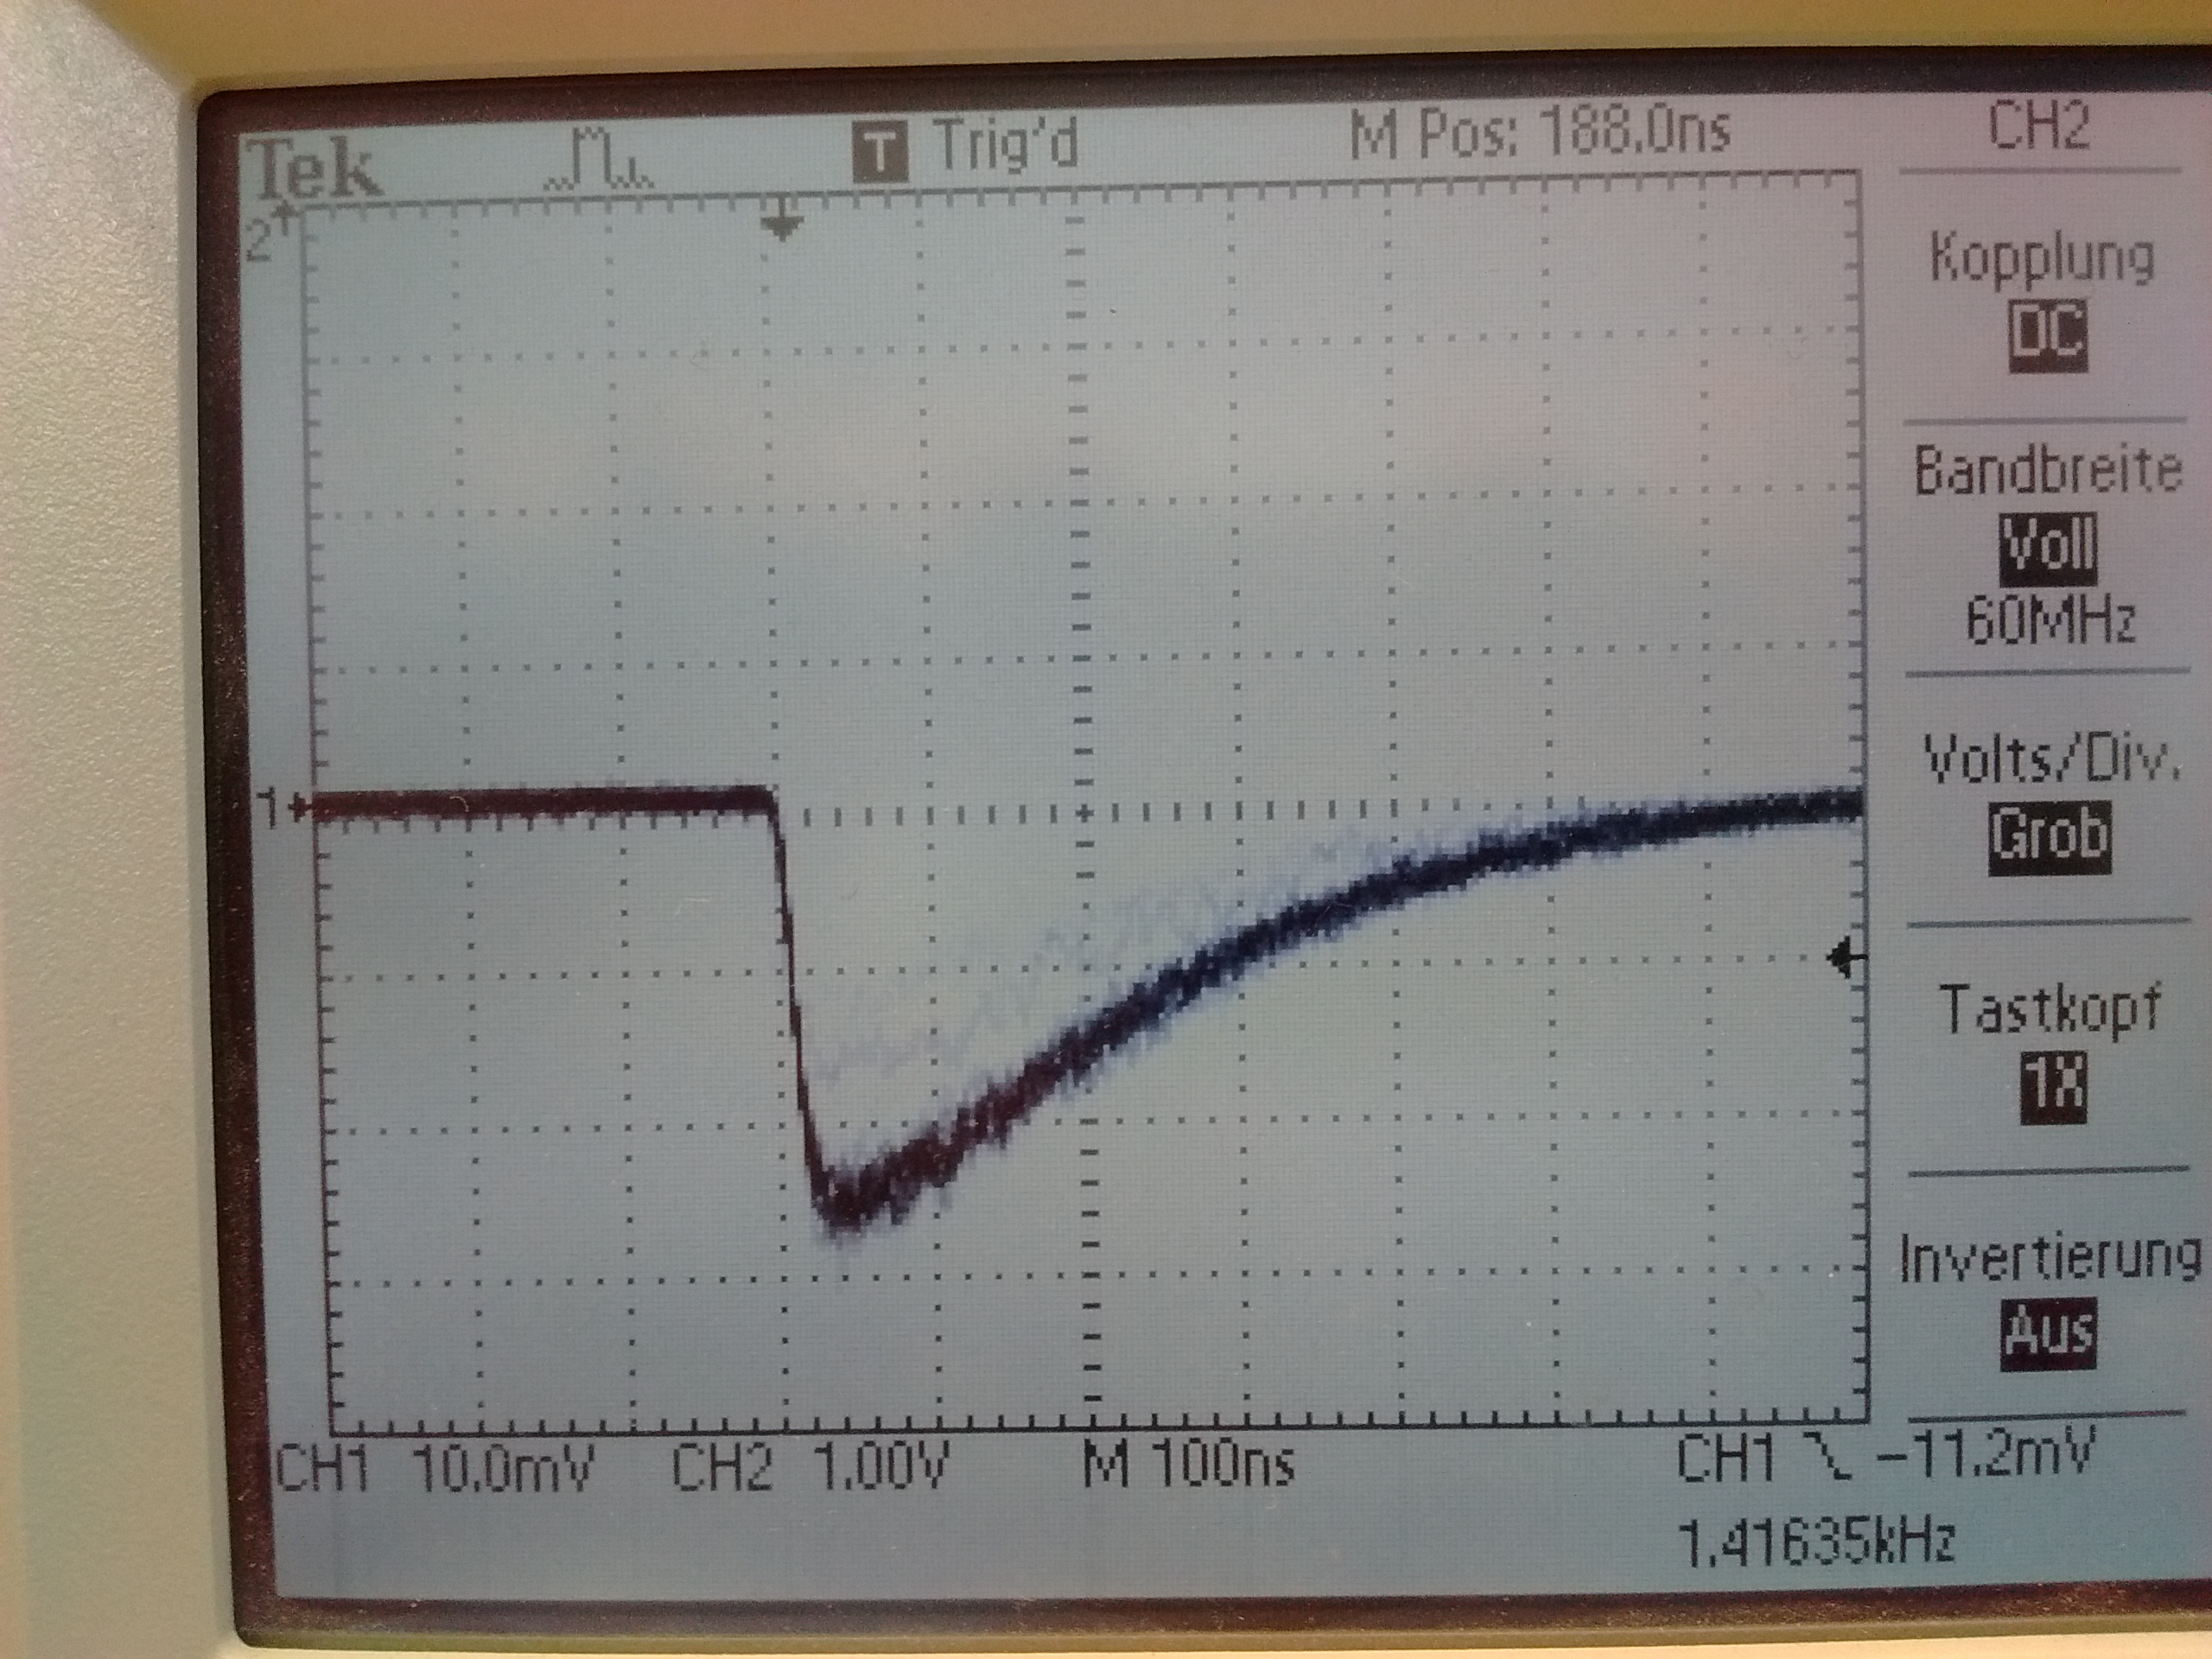
\includegraphics[width=0.5\linewidth]{../graphics/oszi.jpg}
	\caption{%
		Signal des Photomultipliers bei \SI{700}{\volt} Spannung
	}
	\label{fig:oszi}
\end{figure}

Nun verbinden wir den Detektor mit dem Verstärker und diesen mit der MCA-Karte
in Computer. Wir wählen die Verstärkung so, dass der Photopeak des Spektrums
ungefähr bei der Kanal~7000 liegt. Die ersten Messungen nehmen wir mit
einer Lebenszeit (Zeit nach Abzug der Totzeiten) von zehn Minuten auf.
Nun nehmen wir mit unveränderten Aufbau ein Spektrum ohne Absorber (vgl.
Abbildung~\ref{fig:plot_fit_peak_ohne}) in der Mitte
und jeweils ein mit \SI{1,0}{\milli\meter}, \SI{5,0}{\milli\meter},
\SI{10,0}{\milli\meter} und \SI{20,0}{\milli\meter} dicken Aluminiumplättchen
senkrecht zum Strahlengang auf. Die Spektren mit Absorber befinden
sich in Anhang~\ref{anhang-wirkungsquerschnitt}.

Für die Energiekalibrierung stellen wie den Detektor auf den beweglichen Arm
und stellen ihn auf \SI{90}{\degree}. Zunächst nehmen wir eine Untergrund
Messung vor, dann nehmen wir die bekannten Spektren der $^{133}\text{Ba}$- und
der $^{152}\text{Eu}$-Quelle auf. Diese Spektren befinden sich in
Anhang~\ref{anhang-rohspektren-energiekalibrierung}.

Zuletzt wollen wir die Streuspektren der $^{137}\text{Cs}$-Quelle messen. Dafür
entfernen wir die übrigen Quellen und den Bleikollimator, stellen einen Plexiglaszylinder 
in die Mitte. Dieser
sollte auf Grund seiner geringen Kernladungszahl für Comptonstreueffekte besonders
geeignet sein. Nun nehmen wir in dem Bereich von \SIrange{35}{120}{\degree}
in Abständen von \SI{5}{\degree} jeweils fünf Minuten lang das Spektrum auf
(vgl. Anhang~\ref{anhang-streuspektren-untergrund}).

\begin{figure}[h]
    \centering
    \includegraphics[width=\plotwidth]{plot_fit_peak_ohne}
    \caption{%
	    $^{137}\text{Cs}$-Spektrum ohne Aluminium Absorber
   }
    \label{fig:plot_fit_peak_ohne}
\end{figure}



\chapter{Auswertung}

\section{Totaler Wirkungsquerschnitt}

Es werden die Messdaten aus der $^{137}\text{Cs}$-Quelle unter \SI{0}{\degree}
benutzt.
An die Photopeaks der Spektren passen wir eine Gaußfunktion an. Das Resultat
ist vergrößert in Abbildung~\ref{fig:amplituden} zu sehen. Die gesamten
Spektren kann man in Abbildung~\ref{fig:plot_fit_peak_ohne} und im
Anhang~\ref{anhang-wirkungsquerschnitt} betrachten.
\begin{equation}
	g\del x = \frac{a}{\varsigma \sqrt{2 \pi}} \exp\del{\frac{\del
		{x - x_0}^2}{2 \varsigma^2}}
		\quad \quad \quad \text{mit FWHM} \approx 2.355 \varsigma
\end{equation}
Die Flächen unter den Gaußkurven sind auf die Kurve ohne Absorber normiert als
Intensitäten in Tabelle~\ref{tab:amplituden} aufgeführt. An diese wurde in
Abbildung~\ref{fig:cross-section} eine Exponentialfunktion der folgenden Form
angepasst:
\begin{equation}
	N\del x = N_0 \exp\del{-\sigma \rho_T x} \quad \quad \quad \text{mit }
	\rho_T = \frac{N_A \rho}{M}
\end{equation}
Mit dem Ergebnis aus der Anpassung und den Literaturwerten für Aluminium ($\rho
= \SI{<< alu_dichte >>}{\gram\per\cubic\centi\metre}$, $M = \SI{<< alu_amu >>}
{\atomicmassunit}$) ergibt sich für den totalen Wirkungsquerschnitt $\sigma$:
\begin{align*}
	&\sigma \rho_T = \SI{<< alu_a >>}{\per\milli\metre}
	&&\rho_T = \SI{<< alu_n >>}{\per\cubic\milli\metre}
	&&\implies \sigma = \SI{<< alu_sigma >>}{\barn}
\end{align*}

Dieser Wert weicht deutlich von dem aus Altprotokollen erwarteten $\sigma
\approx \SI{0.25}{\barn}$ ab.
Durch den verwendeten Bleikollimator ist der gemessene Winkelbereich sehr klein
und somit auch der Hintergrund zu vernachlässigen.
Die nicht berücksichtigte Detektoreffizienz würde nur zu einem größeren
$\sigma$ führen. So bleiben zur Erklärung nur unbekannte systematische
Fehlerquellen.

\begin{figure}
    \centering
    \includegraphics[width=\plotwidth]{total-cross-section-data}
    \caption{%
	    Photopeaks im Spektrum der eingebauten $^{137}\text{Cs}$-Quelle ohne
	    und mit \SIlist{1;5;10;20}{\milli\meter} Aluminium Absorber
    }
    \label{fig:amplituden}
\end{figure}

\begin{table}
    \centering
    \begin{tabular}{SSSS}
        {Dicke / \si{\milli\meter}} &
        {Scheitelpunkt / Kanal} &
        {FWHM / Kanal} &
	{rel.\ Intensität} \\
        \midrule
        %< for row in total_cross_section_table: ->%
        << ' & '.join(row) >> \\
        %< endfor ->%
    \end{tabular}
    \caption{%
        Anpassungsparameter für die verschiedenen Dicken der
        Absorbermaterialien.
    }
    \label{tab:amplituden}
\end{table}

\begin{figure}
    \centering
    \includegraphics[width=\plotwidth]{total-cross-section-fit}
    \caption{%
	    Transmittierte relative Intensität abhängig von der Absoberdicke
	    mit angepasster Exponentialfunktion
    }
    \label{fig:cross-section}
\end{figure}

\clearpage

\section{Energiekalibrierung}

Mit den Messdaten aus der $^{133}\text{Ba}$- und $^{152}\text{Eu}$ Quelle unter
\SI{90}{\degree} sowie der Messung ohne Absorber aus der
$^{137}\text{Cs}$-Quelle unter \SI{0}{\degree}
wird nun die Energiekalibrierung durchgeführt. Dazu werden, soweit vorhanden,
der Untergründe abgezogen und dann an die Spitzen der
Spektren Gaußfunktionen angepasst. Das Ergebnis ist in
Abbildung~\ref{fig:plot_fit_peak_ohne} und den Abbildungen im
Anhang~\ref{anhang-energiekalibrierung}
zu sehen. Außerdem sind die Parameter der Gaußfunktionen noch einmal in
Tabelle~\ref{tab:energiekalibrierung}
aufgeführt. Mit diesen Werten lässt sich nun eine Energie-Kanal Beziehung
erstellen:
\begin{align}
	E\del x = m x + n
	&&\text{mit } m = \SI{<< energy_slope >>}{\kilo\electronvolt}\text{, }
	\quad n = \SI{<< energy_offset >>}{\kilo\electronvolt}
\end{align}
Dabei wurden die Parameter der in Abbildung~\ref{fig:plot_energy-calibrate-fit}
dargestellten Geraden entnommen. Die Datenpunkte sind mit Fehler dargestellt,
allerdings ist dieser kaum sichtbar. Es gibt keine großen Abweichungen der
Datenpunkte zur angepassten Geraden, so dass wir im folgenden von einer guten
Energiekalibrierung ausgehen.

\begin{figure}
	\centering
	\begin{tabular}{SSS}
		{Scheitelpunkte / Kanal} &
		{FWHM / Kanal} &
		{Energie / \si{\kilo\electronvolt}}\\
		\midrule
		%< for row in energy_calibration_table: ->%
		<< ' & '.join(row) >> \\
		%< endfor ->%
	\end{tabular}
	\caption{%
		Anpassungsparameter für die Energiekalibrierung
	}
	\label{tab:energiekalibrierung}
\end{figure}

\begin{figure}
    \centering
    \includegraphics[width=\plotwidth]{plot_energy-calibrate-fit}
    \caption{%
	    Energiekalibrierung
    }
    \label{fig:plot_energy-calibrate-fit}
\end{figure}


\section{Auswertung der Streuspektren}
\begin{figure}
	\centering
	\begin{tabular}{SSSSS}
		{Winkel} &
		{Scheitelpunkte} &
		{FWHM} &
		{Fläche}&
		{Energie / \si{\kilo\electronvolt}}\\
		\midrule
		%< for row in winkel_energie_table: ->%
		<< ' & '.join(row) >> \\
		%< endfor ->%
	\end{tabular}
	\caption{%
		Anpassungeparameter der Streuspektren unter unterschiedlichen
		Winkeln
	}
	\label{tab:peakanpassung}
\end{figure}

An die untergrundbereinigten Streuspektren wird jeweils eine Gaußfunktion
angepasst, wie in Anhang~\ref{anhang-streuspektren-gauss} zu sehen ist.
Die Parameter dieser Anpassungen sind in Tabelle~\ref{tab:peakanpassung}
zusammengefasst. Mit der vorher erstellten Energiekalibrierung wird jeder
Spitze eine Energie zugewiesen.

\begin{figure}
    \centering
    \includegraphics[width=\plotwidth]{plot_winkel-abh-fit}
    \caption{%
	    Winkelabhängigkeit der Photonenenergie nach Compton-Streuung
    }
    \label{fig:plot_winkel-abh-fit}
\end{figure}

Die Beziehung zwischen Winkel und Energie ist durch die Comptonstreuung
gegeben. Wir gehen von einer Photonenenergie $E_\gamma =
\SI{662}{\kilo\electronvolt}$ aus und tragen in
Abbildung~\ref{fit:plot_winkel-abh-fit} $P$ gegen die Energie der Datenpunkte
auf.
\begin{equation}
	P\del \theta = \frac1{1 +
		\frac{\SI{662}{\kilo\electronvolt}}{\SI{511}{\kilo\electronvolt}}
		\del{1 - \cos\del\theta}}
\end{equation}

Die an die Daten angepasste Gerade sollte der Theorie nach eine Steigung von
$\SI{662}{\kilo\electronvolt}$ aufweisen. Die in
Abbildung~\ref{fig:plot_winkel-abh-fit} gewonnen Parameter sind aber:
\begin{align}
	E\del P = m P + n
	&&\text{mit } m = \SI{<< scatter_energy_slope >>}{\kilo\electronvolt}\text{, }
	\quad n = \SI{<< scatter_energy_offset >>}{\kilo\electronvolt}
\end{align}
Da unsere Energiekalibrierung sehr plausible Ergebnisse liefert gehen wir nicht
von einer verschobenen Energieskala aus. Andere systematische Fehler, die sich
so äußern können, finden wir aber auch nicht.

Als nächstes skalieren wir die Flächen unter den Gaußkurven mit der
Detektoreffizienz aus der Versuchsanleitung. Dazu haben wir einzelne Punkte aus
\parencite[Abbildung P526.3]{physik512-Anleitung} abgelesen und den Bereich
dazwischen mit kubischen Splines
iterpoliert. Das Ergebnis ist in
Abbildung~\ref{fig:plot_fit_anspechwahrscheinlichkeit} zu sehen.
\begin{figure}
    \centering
    \includegraphics[width=\plotwidth]{plot_fit_anspechwahrscheinlichkeit}
    \caption{%
	    Detektoreffizienz aus \parencite[Abbildung
	    P526.3]{physik512-Anleitung}. Datenpunkte
	    abgelesen und mit kubischen Splines interpoliert.
    }
    \label{fig:plot_fit_anspechwahrscheinlichkeit}
\end{figure}

Da wir im ersten Versuchsteil ein Aluminium Absorber verwendet haben hilft uns
das wenig bei der Bestimmung der Absorbtion im Plexiglas. Zur Normierung wird
also jeder Wert einzeln mit einem Klein-Nishina-Graphen zu
$\SI{662}{\kilo\electronvolt}$ verglichen. Daraus erhalten wir Koeffizienten,
die, einzeln mit den korrigierten Intensitäten multipliziert, mit dem
Klein-Nishina-Graphen übereinstimmen. Die Parameter sind in
Tabelle~\ref{tab:klein-nishina-anpassung} zu sehen. Da der verwendete
Plexiglasstab aber rotationssymmetrisch ist gehen wir davon aus, dass alle
Werte mit einem gemeinsamen konstanten Faktor korrigiert werden können.
Das war leider ein Trugschluss, wie in Abbildung~\ref{fig:plot_klein_nishina}
zu sehen ist. Nachdem sich in den vorherigen Versuchsteilen schon starke
Abweichungen von den erwarteten Werten gezeigt haben bleibt nur noch
festzuhalten, dass die Intensität von der Messung bei \SI{50}{\degree} so stark
abweicht, dass sie schon fast wieder zum Graphen passt.
\begin{figure}
	\centering
	\begin{tabular}{SSSS}
		{Winkel} &
		{korr. Intensität} &
		{Koeffizienten}&
		{Energie / \si{\kilo\electronvolt}}\\
		\midrule
		%< for row in scatter_winkel_table: ->%
		<< ' & '.join(row) >> \\
		%< endfor ->%
	\end{tabular}
	\caption{%
		Anpassungeparameter an den Klein-Nishina-Wirkungsquerschnitt
	}
	\label{tab:klein-nishina-anpassung}
\end{figure}

\begin{figure}
    \centering
    \includegraphics[width=\plotwidth]{plot_klein_nishina}
    \caption{%
	    Klein-Nishina-Wirkungsquerschnitt mit skalierten Werten. Die
	    $r$-Achse ist in \si{\milli\barn} dargestellt.
	    Blau: theoretischer Klein-Nichina-Graph.
	    Rot: Datenpunkte
    }
    \label{fig:plot_klein_nishina}
\end{figure}


\chapter{Ergebnis}
Wir konnten im ersten Versuchsteil zwar das Gesetz von Lambert-Beer bestätigen,
allerdings überzeugt uns der ermittelte Wirkungsquerschnitt nicht so sehr.

Auch beim Nachweis des Klein-Nishina-Wirkungsquerschnitts sehen wir Effekte,
die sich nicht nur mit Comptonstreuung erklären lassen. Entweder ist das
Plexiglas doch nicht so gut zum Nachweis von Comptonstreuung geeignet, wie wir
gedacht haben, oder wir haben einen systematischen Fehler im Aufbau, den wir
nicht erklären können.

Insgesamt gesehen ist das also kein sehr befriedigendes Ergebnis.



%TODO


%%%%%%%%%%%%%%%%%%%%%%%%%%%%%%%%%%%%%%%%%%%%%%%%%%%%%%%%%%%%%%%%%%%%%%%%%%%%%%%
%                                   Anhang                                    %
%%%%%%%%%%%%%%%%%%%%%%%%%%%%%%%%%%%%%%%%%%%%%%%%%%%%%%%%%%%%%%%%%%%%%%%%%%%%%%%

\begin{appendix}

\chapter{Anhang}

\section{Abbildungen von Spektren mit Untergrund}\label{anhang-rohspektren-energiekalibrierung}
\begin{figure}[h]
    \centering
    \includegraphics[width=0.65\textwidth]{plot_data_raw_Ba}
    \caption{%
	    $^{133}\text{Ba}$-Spektrum mit Untergrund
    }
    \label{fig:plot_data_raw_Ba}
\end{figure}

\begin{figure}[h]
    \centering
    \includegraphics[width=0.65\textwidth]{plot_data_raw_Eu}
    \caption{%
	    $^{152}\text{Eu}$-Spektrum mit Untergrund
   }
    \label{fig:plot_data_raw_Eu}
\end{figure}

\clearpage

\section{Abbildungen zur Bestimmung des totalen Wirkungsquerschnitts} \label{anhang-wirkungsquerschnitt}
\begin{figure}[h]
    \centering
    \includegraphics[width=0.65\textwidth]{plot_fit_peak_01mm}
    \caption{%
	    $^{137}\text{Cs}$-Spektrum mit \SI{1}{\milli\metre} Aluminium
	    Absorber
    }
    \label{fig:plot_fit_peak_01mm}
\end{figure}

\begin{figure}[h]
    \centering
    \includegraphics[width=0.65\textwidth]{plot_fit_peak_05mm}
    \caption{%
	    $^{137}\text{Cs}$-Spektrum mit \SI{5}{\milli\metre} Aluminium
	    Absorber
   }
    \label{fig:plot_fit_peak_05mm}
\end{figure}

\begin{figure}[h]
    \centering
    \includegraphics[width=0.65\textwidth]{plot_fit_peak_10mm}
    \caption{%
	    $^{137}\text{Cs}$-Spektrum mit \SI{10}{\milli\metre} Aluminium
	    Absorber
   }
    \label{fig:plot_fit_peak_10mm}
\end{figure}

\begin{figure}[h]
    \centering
    \includegraphics[width=0.65\textwidth]{plot_fit_peak_20mm}
    \caption{%
	    $^{137}\text{Cs}$-Spektrum mit \SI{20}{\milli\metre} Aluminium
	    Absorber
   }
    \label{fig:plot_fit_peak_20mm}
\end{figure}

\clearpage

\section{Abbildungen zur Energiekalibrierung} \label{anhang-energiekalibrierung}
\begin{figure}[h]
    \centering
    \includegraphics[width=0.65\textwidth]{plot_peaks_Ba}
    \caption{%
	    Untergrundbereinigtes $^{133}\text{Ba}$-Spektrum mit
	    Gaußanpassungen
   }
    \label{fig:plot_peaks_Ba}
\end{figure}

\begin{figure}[h]
    \centering
    \includegraphics[width=0.65\textwidth]{plot_peaks_Eu}
    \caption{%
	    Untergrundbereinigtes $^{152}\text{Eu}$-Spektrum mit
	    Gaußanpassungen
    }
    \label{fig:plot_peaks_Eu}
\end{figure}

\clearpage

\section{Abbildungen zu den einzelnen Winkeln}\label{anhang-streuspektren}
\subsection{Streuspektren mit Untergrund}
\label{anhang-streuspektren-untergrund}
\begin{figure}[h]
    \centering
    \includegraphics[width=0.65\textwidth]{plot_raw_w035}
    \caption{%
	    Streuspektrum mit Untergrund bei \SI{35}{\degree}
    }
    \label{fig:plot_raw_w035}
\end{figure}

\begin{figure}[h]
    \centering
    \includegraphics[width=0.65\textwidth]{plot_raw_w040}
    \caption{%
	    Streuspektrum mit Untergrund bei \SI{40}{\degree}
    }
    \label{fig:plot_raw_w040}
\end{figure}

\begin{figure}[h]
    \centering
    \includegraphics[width=0.65\textwidth]{plot_raw_w045}
    \caption{%
	    Streuspektrum mit Untergrund bei \SI{45}{\degree}
    }
    \label{fig:plot_raw_w045}
\end{figure}

\begin{figure}[h]
    \centering
    \includegraphics[width=0.65\textwidth]{plot_raw_w050}
    \caption{%
	    Streuspektrum mit Untergrund bei \SI{50}{\degree}
    }
    \label{fig:plot_raw_w050}
\end{figure}

\begin{figure}[h]
    \centering
    \includegraphics[width=0.65\textwidth]{plot_raw_w055}
    \caption{%
	    Streuspektrum mit Untergrund bei \SI{55}{\degree}
    }
    \label{fig:plot_raw_w055}
\end{figure}

\begin{figure}[h]
    \centering
    \includegraphics[width=0.65\textwidth]{plot_raw_w060}
    \caption{%
	    Streuspektrum mit Untergrund bei \SI{60}{\degree}
    }
    \label{fig:plot_raw_w060}
\end{figure}

\begin{figure}[h]
    \centering
    \includegraphics[width=0.65\textwidth]{plot_raw_w065}
    \caption{%
	    Streuspektrum mit Untergrund bei \SI{65}{\degree}
    }
    \label{fig:plot_raw_w065}
\end{figure}

\begin{figure}[h]
    \centering
    \includegraphics[width=0.65\textwidth]{plot_raw_w070}
    \caption{%
	    Streuspektrum mit Untergrund bei \SI{70}{\degree}
    }
    \label{fig:plot_raw_w070}
\end{figure}

\begin{figure}[h]
    \centering
    \includegraphics[width=0.65\textwidth]{plot_raw_w075}
    \caption{%
	    Streuspektrum mit Untergrund bei \SI{75}{\degree}
    }
    \label{fig:plot_raw_w075}
\end{figure}

\begin{figure}[h]
    \centering
    \includegraphics[width=0.65\textwidth]{plot_raw_w080}
    \caption{%
	    Streuspektrum mit Untergrund bei \SI{80}{\degree}
    }
    \label{fig:plot_raw_w080}
\end{figure}

\begin{figure}[h]
    \centering
    \includegraphics[width=0.65\textwidth]{plot_raw_w085}
    \caption{%
	    Streuspektrum mit Untergrund bei \SI{85}{\degree}
    }
    \label{fig:plot_raw_w085}
\end{figure}

\begin{figure}[h]
    \centering
    \includegraphics[width=0.65\textwidth]{plot_raw_w090}
    \caption{%
	    Streuspektrum mit Untergrund bei \SI{90}{\degree}
    }
    \label{fig:plot_raw_w090}
\end{figure}

\begin{figure}[h]
    \centering
    \includegraphics[width=0.65\textwidth]{plot_raw_w095}
    \caption{%
	    Streuspektrum mit Untergrund bei \SI{95}{\degree}
    }
    \label{fig:plot_raw_w095}
\end{figure}

\begin{figure}[h]
    \centering
    \includegraphics[width=0.65\textwidth]{plot_raw_w100}
    \caption{%
	    Streuspektrum mit Untergrund bei \SI{100}{\degree}
    }
    \label{fig:plot_raw_w100}
\end{figure}

\begin{figure}[h]
    \centering
    \includegraphics[width=0.65\textwidth]{plot_raw_w105}
    \caption{%
	    Streuspektrum mit Untergrund bei \SI{105}{\degree}
    }
    \label{fig:plot_raw_w105}
\end{figure}

\begin{figure}[h]
    \centering
    \includegraphics[width=0.65\textwidth]{plot_raw_w110}
    \caption{%
	    Streuspektrum mit Untergrund bei \SI{110}{\degree}
    }
    \label{fig:plot_raw_w110}
\end{figure}

\begin{figure}[h]
    \centering
    \includegraphics[width=0.65\textwidth]{plot_raw_w115}
    \caption{%
	    Streuspektrum mit Untergrund bei \SI{115}{\degree}
    }
    \label{fig:plot_raw_w115}
\end{figure}

\begin{figure}[h]
    \centering
    \includegraphics[width=0.65\textwidth]{plot_raw_w120}
    \caption{%
	    Streuspektrum mit Untergrund bei \SI{120}{\degree}
    }
    \label{fig:plot_raw_w120}
\end{figure}

\clearpage

\subsection{Streuspektren mit Gaußanpassungen}
\label{anhang-streuspektren-gauss}
\begin{figure}[h]
    \centering
    \includegraphics[width=0.65\textwidth]{plot_anpassung_w035}
    \caption{%
	    Streuspektrum mit Gaußanpassungen bei \SI{35}{\degree}
    }
    \label{fig:plot_anpassung_w035}
\end{figure}

\begin{figure}[h]
    \centering
    \includegraphics[width=0.65\textwidth]{plot_anpassung_w040}
    \caption{%
	    Streuspektrum mit Gaußanpassungen bei \SI{40}{\degree}
    }
    \label{fig:plot_anpassung_w040}
\end{figure}

\begin{figure}[h]
    \centering
    \includegraphics[width=0.65\textwidth]{plot_anpassung_w045}
    \caption{%
	    Streuspektrum mit Gaußanpassungen bei \SI{45}{\degree}
    }
    \label{fig:plot_anpassung_w045}
\end{figure}

\begin{figure}[h]
    \centering
    \includegraphics[width=0.65\textwidth]{plot_anpassung_w050}
    \caption{%
	    Streuspektrum mit Gaußanpassungen bei \SI{50}{\degree}
    }
    \label{fig:plot_anpassung_w050}
\end{figure}

\begin{figure}[h]
    \centering
    \includegraphics[width=0.65\textwidth]{plot_anpassung_w055}
    \caption{%
	    Streuspektrum mit Gaußanpassungen bei \SI{55}{\degree}
    }
    \label{fig:plot_anpassung_w055}
\end{figure}

\begin{figure}[h]
    \centering
    \includegraphics[width=0.65\textwidth]{plot_anpassung_w060}
    \caption{%
	    Streuspektrum mit Gaußanpassungen bei \SI{60}{\degree}
    }
    \label{fig:plot_anpassung_w060}
\end{figure}

\begin{figure}[h]
    \centering
    \includegraphics[width=0.65\textwidth]{plot_anpassung_w065}
    \caption{%
	    Streuspektrum mit Gaußanpassungen bei \SI{65}{\degree}
    }
    \label{fig:plot_anpassung_w065}
\end{figure}

\begin{figure}[h]
    \centering
    \includegraphics[width=0.65\textwidth]{plot_anpassung_w070}
    \caption{%
	    Streuspektrum mit Gaußanpassungen bei \SI{70}{\degree}
    }
    \label{fig:plot_anpassung_w070}
\end{figure}

\begin{figure}[h]
    \centering
    \includegraphics[width=0.65\textwidth]{plot_anpassung_w075}
    \caption{%
	    Streuspektrum mit Gaußanpassungen bei \SI{75}{\degree}
    }
    \label{fig:plot_anpassung_w075}
\end{figure}

\begin{figure}[h]
    \centering
    \includegraphics[width=0.65\textwidth]{plot_anpassung_w080}
    \caption{%
	    Streuspektrum mit Gaußanpassungen bei \SI{80}{\degree}
    }
    \label{fig:plot_anpassung_w080}
\end{figure}

\begin{figure}[h]
    \centering
    \includegraphics[width=0.65\textwidth]{plot_anpassung_w085}
    \caption{%
	    Streuspektrum mit Gaußanpassungen bei \SI{85}{\degree}
    }
    \label{fig:plot_anpassung_w085}
\end{figure}

\begin{figure}[h]
    \centering
    \includegraphics[width=0.65\textwidth]{plot_anpassung_w090}
    \caption{%
	    Streuspektrum mit Gaußanpassungen bei \SI{90}{\degree}
    }
    \label{fig:plot_anpassung_w090}
\end{figure}

\begin{figure}[h]
    \centering
    \includegraphics[width=0.65\textwidth]{plot_anpassung_w095}
    \caption{%
	    Streuspektrum mit Gaußanpassungen bei \SI{95}{\degree}
    }
    \label{fig:plot_anpassung_w095}
\end{figure}

\begin{figure}[h]
    \centering
    \includegraphics[width=0.65\textwidth]{plot_anpassung_w100}
    \caption{%
	    Streuspektrum mit Gaußanpassungen bei \SI{100}{\degree}
    }
    \label{fig:plot_anpassung_w100}
\end{figure}

\begin{figure}[h]
    \centering
    \includegraphics[width=0.65\textwidth]{plot_anpassung_w105}
    \caption{%
	    Streuspektrum mit Gaußanpassungen bei \SI{105}{\degree}
    }
    \label{fig:plot_anpassung_w105}
\end{figure}

\begin{figure}[h]
    \centering
    \includegraphics[width=0.65\textwidth]{plot_anpassung_w110}
    \caption{%
	    Streuspektrum mit Gaußanpassungen bei \SI{110}{\degree}
    }
    \label{fig:plot_anpassung_w110}
\end{figure}

\begin{figure}[h]
    \centering
    \includegraphics[width=0.65\textwidth]{plot_anpassung_w115}
    \caption{%
	    Streuspektrum mit Gaußanpassungen bei \SI{115}{\degree}
    }
    \label{fig:plot_anpassung_w115}
\end{figure}

\begin{figure}[h]
    \centering
    \includegraphics[width=0.65\textwidth]{plot_anpassung_w120}
    \caption{%
	    Streuspektrum mit Gaußanpassungen bei \SI{120}{\degree}
    }
    \label{fig:plot_anpassung_w120}
\end{figure}

\clearpage


%TODO

\end{appendix}

\end{document}

% vim: spell spelllang=de tw=79
